% -----------------------------*- LaTeX -*------------------------------
\documentclass[UTF8]{report}
% ------------------------------------------------------------------------
% Packages
% ------------------------------------------------------------------------
\usepackage{ctex} % 支持中文
\usepackage[body={7in, 9in},left=1in,right=1in]{geometry} % 改变页边距
\usepackage{amsmath} % AMS 的数学宏包
\usepackage{amsfonts} % AMS 的数学字体宏包
\usepackage{amssymb} % AMS 符号库
\usepackage{bm} % 数学公式中的黑斜体h
\usepackage{amsthm} % AMS 的定理环境宏包
\usepackage{graphicx} % 插图
\usepackage{subfigure} % 插子图
\usepackage{nicefrac} % 好看的分数
\usepackage{mathrsfs} % mathscr font
\usepackage{caption} % caption
\usepackage{algorithm,algorithmicx} % 伪代码支持宏包
\usepackage[noend]{algpseudocode} % 伪代码
\usepackage{fancyhdr} % 设置页眉、页脚
\usepackage{adjustbox} % 图片尺寸自动调整
\usepackage{esint} % 积分符号
\usepackage{mathtools} % 数学宏包的重要补充
\usepackage{upgreek} % 数学环境的直立希腊字母
\usepackage{enumitem} % 使用enumitem宏包, 改变列表项的格式
\usepackage{color} % 支持彩色
\usepackage{extarrows} % 任意长度的箭头
\usepackage{tikz} % 绘图
\usepackage{forest} % 绘树
\usepackage{xcolor} % 颜色宏包
\usepackage{breqn} % 公式自动换行
\usepackage{fontsize} % 字体大小
\usepackage[framemethod=TikZ]{mdframed} % 给文字加框
\usepackage{fontspec} % 字体库
\usepackage{bigstrut} % 用于表格中的换行
\usepackage{multirow} % 表格中多行单元格合并
\usepackage{multicol} % 表格中多列单元格合并
\usepackage{longtable} % 长表格
\usepackage{rotating} % 旋转图形和表格      以上三者用于绘制三线表
\usepackage{booktabs} % 三线表宏包
\usepackage{forest} % 绘制语法树
\usepackage{scribe} % Scribe 模板
\usepackage{diagbox} % 表格斜线
\usepackage{listings} % 插入代码
\usepackage{verbatim} % 多行注释
\usepackage{ifplatform} % 检测编译平台
\usepackage{hyperref} % 超链接
\usepackage{mathrsfs} % 花体
\usepackage{pgffor} % foreach
\usepackage{circuitikz} % 画电路图
\usepackage{svg} % 插入svg
\usetikzlibrary{shapes.geometric, arrows} % 引入流程图需要的库
\usetikzlibrary{automata} % 引入automata库
\usetikzlibrary{shapes,arrows,positioning,chains} % 引入positioning库
% ------------------------------------------------------------------------
% Macros
% ------------------------------------------------------------------------
%~~~~~~~~~~~~~~~
% Utility latin
%~~~~~~~~~~~~~~~
\newcommand{\ie}{\textit{i.e.}}
\newcommand{\eg}{\textit{e.g.}}
%~~~~~~~~~~~~~~~
% Environment shortcuts
%~~~~~~~~~~~~~~~
\newcommand{\balign}[1]{\ealign{\begin{align}#1\end{align}}}
\newcommand{\baligns}[1]{\ealigns{\begin{align*}#1\end{align*}}}
\newcommand{\bitemize}[1]{\eitemize{\begin{itemize}#1\end{itemize}}}
\newcommand{\benumerate}[1]{\eenumerate{\begin{enumerate}#1\end{enumerate}}}
%~~~~~~~~~~~~~~~
% Text with quads around it
%~~~~~~~~~~~~~~~
\newcommand{\qtext}[1]{\quad\text{#1}\quad}
%~~~~~~~~~~~~~~~
% Shorthand for math formatting
%~~~~~~~~~~~~~~~
\newcommand{\mbb}[1]{\mathbb{#1}}
\newcommand{\mbi}[1]{\boldsymbol{#1}} % Bold and italic (math bold italic)
\newcommand{\mbf}[1]{\mathbf{#1}}
\newcommand{\mc}[1]{\mathcal{#1}}
\newcommand{\mrm}[1]{\mathrm{#1}}
\newcommand{\tbf}[1]{\textbf{#1}}
\newcommand{\tsc}[1]{\textsc{#1}}
%\def\\langle {{\langle }}
%\def\\rangle {{\rangle }}
\newcommand{\sT}{\sf T}
\newcommand{\grad}{\nabla}
\newcommand{\Proj}{\Pi}
%~~~~~~~~~~~~~~~
% Common sets 定义数集符号
%~~~~~~~~~~~~~~~
\newcommand{\R}{\mathbb{R}}
\newcommand{\Z}{\mathbb{Z}}
\newcommand{\Q}{\mathbb{Q}}
\newcommand{\N}{\mathbb{N}}
\newcommand{\C}{\mathbb{C}}
\newcommand{\reals}{\mathbb{R}} % Real number symbol
\newcommand{\integers}{\mathbb{Z}} % Integer symbol
\newcommand{\rationals}{\mathbb{Q}} % Rational numbers
\newcommand{\naturals}{\mathbb{N}} % Natural numbers
\newcommand{\complex}{\mathbb{C}} % Complex numbers
%~~~~~~~~~~~~~~~
% Common functions
%~~~~~~~~~~~~~~~
\renewcommand{\exp}[1]{\operatorname{exp}\left(#1\right)} % Exponential
\newcommand{\indic}[1]{\mbb{I}\left(#1\right)} % Indicator function
\newcommand{\indicsub}[2]{\mbb{I}_{#2}\left(#1\right)} % Indicator function
\newcommand{\argmax}{\mathop\mathrm{arg\, max}} % Defining math symbols
\newcommand{\argmin}{\mathop\mathrm{arg\, min}}
\renewcommand{\arccos}{\mathop\mathrm{arccos}}
\newcommand{\dom}{\mathop\mathrm{dom}} % Domain
\newcommand{\range}{\mathop\mathrm{range}} % Range
\newcommand{\diag}{\mathop\mathrm{diag}}
\newcommand{\tr}{\mathop\mathrm{tr}}
\newcommand{\abs}{\mathop\mathrm{abs}}
\newcommand{\card}{\mathop\mathrm{card}}
\newcommand{\sign}{\mathop\mathrm{sign}}
\newcommand{\prox}{\mathrm{prox}} % prox
\newcommand{\rank}[1]{\mathrm{rank}(#1)}
\newcommand{\supp}[1]{\mathrm{supp}(#1)}
\newcommand{\norm}[1]{\lVert#1\rVert}
%~~~~~~~~~~~~~~~
% Common probability symbols
%~~~~~~~~~~~~~~~
\newcommand{\family}{\mathcal{P}} % probability family / statistical model
\newcommand{\iid}{\stackrel{\mathrm{iid}}{\sim}}
\newcommand{\ind}{\stackrel{\mathrm{ind}}{\sim}}
\newcommand{\E}{\mathbb{E}} % Expectation symbol
\newcommand{\Earg}[1]{\E\left[#1\right]}
\newcommand{\Esubarg}[2]{\E_{#1}\left[#2\right]}
\renewcommand{\P}{\mathbb{P}} % Probability symbol
\newcommand{\Parg}[1]{\P\left(#1\right)}
\newcommand{\Psubarg}[2]{\P_{#1}\left[#2\right]}
%\newcommand{\Cov}{\mrm{Cov}} % Covariance symbol
%\newcommand{\Covarg}[1]{\Cov\left[#1\right]}
%\newcommand{\Covsubarg}[2]{\Cov_{#1}\left[#2\right]}
%\newcommand{\model}{\mathcal{P}} % probability family / statistical model
%~~~~~~~~~~~~~~~
% Distributions
%~~~~~~~~~~~~~~~
%\newcommand{\Gsn}{\mathcal{N}}
%\newcommand{\Ber}{\textnormal{Ber}}
%\newcommand{\Bin}{\textnormal{Bin}}
%\newcommand{\Unif}{\textnormal{Unif}}
%\newcommand{\Mult}{\textnormal{Mult}}
%\newcommand{\NegMult}{\textnormal{NegMult}}
%\newcommand{\Dir}{\textnormal{Dir}}
%\newcommand{\Bet}{\textnormal{Beta}}
%\newcommand{\Gam}{\textnormal{Gamma}}
%\newcommand{\Poi}{\textnormal{Poi}}
%\newcommand{\HypGeo}{\textnormal{HypGeo}}
%\newcommand{\GEM}{\textnormal{GEM}}
%\newcommand{\BP}{\textnormal{BP}}
%\newcommand{\DP}{\textnormal{DP}}
%\newcommand{\BeP}{\textnormal{BeP}}
%\newcommand{\Exp}{\textnormal{Exp}}
%~~~~~~~~~~~~~~~
% Theorem-like environments
%~~~~~~~~~~~~~~~
%\theoremstyle{definition}
%\newtheorem{definition}{Definition}
%\newtheorem{example}{Example}
%\newtheorem{problem}{Problem}
%\newtheorem{lemma}{Lemma}
%~~~~~~~~~~~~~~~
% 组合数学的模板和作业里用到的一些宏包和自定义命令
%~~~~~~~~~~~~~~~
\renewcommand{\emph}[1]{\begin{kaishu}#1\end{kaishu}}
\newcommand{\falfac}[1]{^{\underline{#1}}}
\newcommand{\binomfrac}[2]{\frac{#1^{\underline{#2}}}{#2!}}
\newcommand{\ceil}[1]{\left\lceil #1 \right\rceil}
\newcommand{\floor}[1]{\left\lfloor #1 \right\rfloor}
\newcommand{\suminfty}[2]{\sum_{#1=#2}^{\infty}}
\newcommand{\suminftyk}[0]{\sum_{k=0}^{\infty}}
\newcommand{\sumint}[3]{\sum_{#1=#2}^{#3}}
\newcommand{\sumintk}[2]{\sum_{k=#1}^{#2}}
\newcommand{\suminti}[2]{\sum_{i=#1}^{#2}}
%~~~~~~~~~~~~~~~
% 定义新命令
%~~~~~~~~~~~~~~~
\newcommand*{\unit}[1]{\mathop{}\!\mathrm{#1}}
\newcommand*{\dif}{\mathop{}\!\mathrm{d}}%微分算子 d
\newcommand*{\pdif}{\mathop{}\!\partial}%偏微分算子
\newcommand*{\cdif}{\mathop{}\!\nabla}%协变导数、nabla 算子
\newcommand*{\laplace}{\mathop{}\!\Delta}%laplace 算子
\newcommand*{\deri}[1]{\mathrm{d} #1}
\newcommand*{\deriv}[2]{\frac{\mathrm{d} #1}{\mathrm{d} {#2}}}
\newcommand*{\derivh}[3]{\frac{\mathrm{d}^{#1} #2}{\mathrm{d} {#3^{#1}}}}
\newcommand*{\pderiv}[2]{\frac{\partial #1}{\partial {#2}}}
\newcommand*{\pderivh}[3]{\frac{\partial^{#1} #2}{\partial {#3^{#1}}}}
\newcommand*{\dderiv}[2]{\dfrac{\mathrm{d} #1}{\mathrm{d} {#2}}}
\newcommand*{\dderivh}[3]{\dfrac{\mathrm{d}^{#1} #2}{\mathrm{d} {#3^{#1}}}}
\newcommand*{\dpderiv}[2]{\dfrac{\partial #1}{\partial {#2}}}
\newcommand*{\dpderivh}[3]{\dfrac{\partial^{#1} #2}{\partial {#3^{#1}}}}
\newcommand{\me}[1]{\mathrm{e}^{#1}}%e 指数
\newcommand{\mi}{\mathrm{i}}%虚数单位
%\newcommand{\mc}{\mathrm{c}}%光速 定义与mathcal冲突
\newcommand{\red}[1]{\textcolor{red}{#1}}
\newcommand{\blue}[1]{\textcolor{blue}{#1}}
%\newcommand{\Rome}[1]{\setcounter{rome}{#1}\Roman{rome}}
%~~~~~~~~~~~~~~~
% 公式环境中箭头符号的简写
%~~~~~~~~~~~~~~~
\newcommand{\ra}{\rightarrow}
\newcommand{\Ra}{\Rightarrow}
\newcommand{\la}{\leftarrow}
\newcommand{\La}{\Leftarrow}
\newcommand{\lra}{\leftrightarrow}
\newcommand{\Lra}{\Leftrightarrow}
\newcommand{\lgla}{\longleftarrow}
\newcommand{\Lgla}{\Longleftarrow}
\newcommand{\lgra}{\longrightarrow}
\newcommand{\Lgra}{\Longrightarrow}
\newcommand{\lglra}{\longleftrightarrow}
\newcommand{\Lglra}{\Longleftrightarrow}
%~~~~~~~~~~~~~~~
% 一些数学的环境设置
%~~~~~~~~~~~~~~~
%\newcounter{counter_exm}\setcounter{counter_exm}{1}
%\newcounter{counter_prb}\setcounter{counter_prb}{1}
%\newcounter{counter_thm}\setcounter{counter_thm}{1}
%\newcounter{counter_lma}\setcounter{counter_lma}{1}
%\newcounter{counter_dft}\setcounter{counter_dft}{1}
%\newcounter{counter_clm}\setcounter{counter_clm}{1}
%\newcounter{counter_cly}\setcounter{counter_cly}{1}
\newtheorem{theorem}{{\hskip 1.7em \bf 定理}}
\newtheorem{lemma}[theorem]{\hskip 1.7em 引理}
\newtheorem{proposition}[theorem]{\hskip 1.7em 命题}
\newtheorem{claim}[theorem]{\hskip 1.7em 断言}
\newtheorem{corollary}[theorem]{\hskip 1.7em 推论}
% \newcommand{\problem}[1]{{\setlength{\parskip}{10pt}\noindent \bf{#1}}}
\newenvironment{solution}{{\noindent \bf 解 \quad}}{}
\newenvironment{remark}{{\noindent \bf 注 \quad}}{}
\newenvironment{definition}{{\noindent \bf 定义 \quad}}{}
\renewenvironment{proof}{{\setlength{\parskip}{7pt}\noindent\hskip 2em \bf 证明 \quad}}{\hfill$\qed$\par}
\newenvironment{example}{{\noindent\bf 例 \quad}}{\hfill$\qed$\par}
%\newenvironment{concept}[1]{{\bf #1\quad} \begin{kaishu}} {\end{kaishu}\par}
%~~~~~~~~~~~~~~~
% 本.tex文档中特殊定义命令
%~~~~~~~~~~~~~~~
\newcommand{\lno}[1]{\overline{#1}}
\newcommand{\NP}{\mathrm{NP}}
\newcommand{\coNP}{\mathrm{coNP}}
% \newcommand{\ISO}{\mathrm{ISO}}
\newcommand{\SAT}{\mathrm{SAT}}
\newcommand{\USAT}{\mathrm{USAT}}
% \newcommand{\threeSAT}{\mathrm{3\text{-}SAT}}
\renewcommand{\P}{\mathrm{P}}
% \mathchardef\mhyphen="2D
% \newcommand{\CNF}{\mathrm{CNF}}
% \newcommand{\DNF}{\mathrm{DNF}}
% \newcommand{\SetSp}{\mathrm{SET\text{-}SPLITTING}}
% \newcommand{\PUZZLE}{\mathrm{PUZZLE}}
% \newcommand{\SPATH}{\mathrm{SPATH}}
% \newcommand{\LPATH}{\mathrm{LPATH}}
% \newcommand{\UHAMPATH}{\mathrm{UHAMPATH}}
\newcommand{\SPACE}{\mathrm{SPACE}}
\newcommand{\NSPACE}{\mathrm{NSPACE}}
\newcommand{\PSPACE}{\mathrm{PSPACE}}
\newcommand{\NPSPACE}{\mathrm{NPSPACE}}
\newcommand{\DFA}{\mathrm{DFA}}
\newcommand{\NFA}{\mathrm{NFA}}
\newcommand{\TQBF}{\mathrm{TQBF}}
% \newcommand{\L}{\mathrm{L}}
\renewcommand{\O}{\mathrm{O}}
\newcommand{\NL}{\mathrm{NL}}
\newcommand{\coNL}{\mathrm{coNL}}
\newcommand{\LADDER}{\mathrm{LADDER_{DFA}}}
\newcommand{\hd}{\mathrm{\text{-}hard}}
\newcommand{\ADD}{\mathrm{ADD}}
\newcommand{\STCN}{\mathrm{STRONGLY\text{-}CONNECTED}}
\newcommand{\PATH}{\mathrm{PATH}}
\newcommand{\A}{\mathrm{A}}
%使用align环境公式换页
\allowdisplaybreaks[4]

\definecolor{dkgreen}{rgb}{0,0.6,0}
\definecolor{gray}{rgb}{0.5,0.5,0.5}
\definecolor{mauve}{rgb}{0.58,0,0.82}
\lstset{
  frame=tb,
  aboveskip=3mm,
  belowskip=3mm,
  showstringspaces=false,
  columns=flexible,
  framerule=1pt,
  rulecolor=\color{gray!35},
  backgroundcolor=\color{gray!5},
  basicstyle={\small\ttfamily},
  numbers=left,
  numberstyle=\ttfamily\color{gray},
  keywordstyle=\color{blue},
  commentstyle=\color{dkgreen},
  stringstyle=\color{mauve},
  breaklines=true,
  breakatwhitespace=true,
  tabsize=3,
}

\lstdefinelanguage{LoongArch}{
  morekeywords={la, lw, addi, sw, li, syscall, beqz, add, move, bge, blt, b, sub, ret, beq, bne},  
  literate={ll.w}{{{\color{blue}ll.w}}}1
           {sc.w}{{{\color{blue}sc.w}}}1
           {addi.d}{{{\color{blue}addi.d}}}1
           {st.d}{{{\color{blue}st.d}}}1
           {st.w}{{{\color{blue}st.w}}}1
           {ldptr.w}{{{\color{blue}ldptr.w}}}1
           {slli.d}{{{\color{blue}slli.d}}}1
           {ld.d}{{{\color{blue}ld.d}}}1
           {stptr.w}{{{\color{blue}stptr.w}}}1
           {slli.w}{{{\color{blue}slli.w}}}1
           {ld.w}{{{\color{blue}ld.w}}}1
           {addi.w}{{{\color{blue}addi.w}}}1
           {add.d}{{{\color{blue}add.d}}}1
           {sub.w}{{{\color{blue}sub.w}}}1
           {li.w}{{{\color{blue}li.w}}}1
           {bstrpick.d}{{{\color{blue}bstrpick.d}}}1
           {alsl.d}{{{\color{blue}alsl.d}}}1,
  morecomment=[l]{\#},
  frame=tb,
  aboveskip=3mm,
  belowskip=3mm,
  showstringspaces=false,
  columns=flexible,
  framerule=1pt,
  rulecolor=\color{gray!35},
  backgroundcolor=\color{gray!5},
  basicstyle={\small\ttfamily},
  numbers=left,
  numberstyle=\ttfamily\color{gray},
  keywordstyle=\color{blue},
  commentstyle=\color{dkgreen},
  stringstyle=\color{mauve},
  breaklines=true,
  breakatwhitespace=true,
  tabsize=3,
}

% 设置超链接样式
\hypersetup{
    colorlinks=true,       % 将链接颜色设置为 true
    linkcolor=magenta,        % 内部链接颜色
    filecolor=magenta,     % 文件链接颜色
    urlcolor=blue,         % URL 链接颜色
    citecolor=green,       % 引用链接颜色
}

\tikzstyle{startstop} = [rectangle, rounded corners, minimum width=3cm, minimum height=1cm,text centered, draw=black, fill=red!30]
\tikzstyle{process} = [rectangle, minimum width=3cm, minimum height=1cm, text centered, draw=black, fill=orange!30]
\tikzstyle{decision} = [diamond, minimum width=3cm, minimum height=1cm, text centered, draw=black, fill=green!30]
\tikzstyle{arrow} = [thick,->,>=stealth]

\ifwindows
    \setmainfont{Times New Roman}
    \setsansfont{Times New Roman}
    \setmonofont{Consolas}
    \setCJKmainfont{SimHei}
    \setCJKsansfont{SimSun}
    \setCJKmonofont{FangSong}
\else
    \setmainfont{Times New Roman}
    \setsansfont{Times New Roman}
    \setmonofont{Menlo}
    \setCJKmainfont{Songti SC}
    \setCJKsansfont{STSong}
    \setCJKmonofont{STFangsong}
\fi

\punctstyle{kaiming}

\begin{document}

\pagestyle{fancy}

\reporttype{Homework}                 % required
\course{Compiler Principle} 				% optional
\coursetitle{中间代码生成}	    % optional
\semester{Spring 2025}			    % optional
\lecturer{Feng Xiaobing}			% optional
\scribe{2022K8009929010 Zhang Jiawei}			% required
\lecturenumber{8}				% required (must be a number)
\lecturedate{May 12}			% required (omit year)
\maketitle

\noindent
\tbf{8.1}

画出DAG如下图所示:

% 可插入到 document 环境中
\begin{center}
    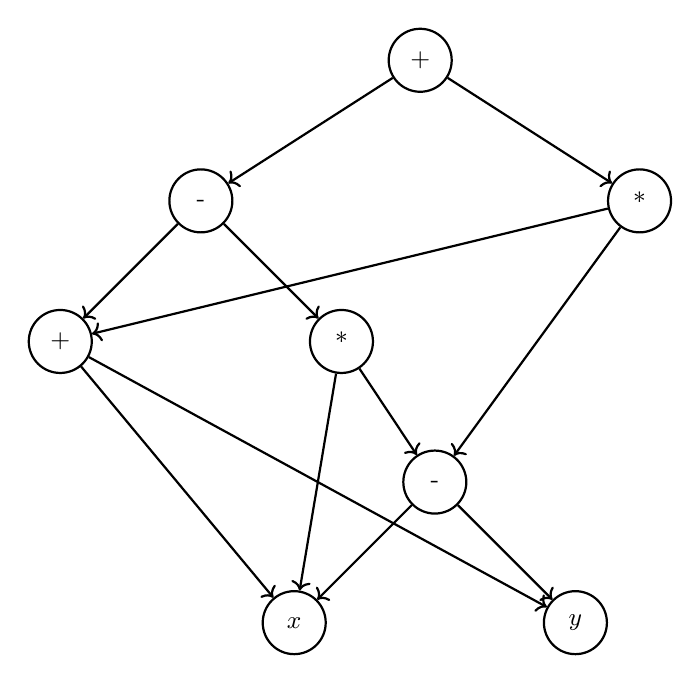
\begin{tikzpicture}[node distance=1.6cm, every node/.style={draw, circle, minimum size=0.8cm, font=\small}, thick]
        % 第一层
        \node (plus1) {+};
        % 第二层
        \node (minus1) [below left=1.2cm and 2.2cm of plus1] {-};
        \node (times2) [below right=1.2cm and 2.2cm of plus1] {*};
        % 第三层
        \node (plus2) [below left=1.2cm and 1.2cm of minus1] {+};
        \node (times1) [below right=1.2cm and 1.2cm of minus1] {*};
        % 第四层
        \node (minus2) [below right=1.2cm and 0.6cm of times1] {-};
        % 第五层        
        \node (x) [below left=1.2cm and 1.2cm of minus2] {$x$};
        \node (y) [below right=1.2cm and 1.2cm of minus2] {$y$};
    
        % 连线
        \draw[->] (plus1) -- (minus1);
        \draw[->] (plus1) -- (times2);
    
        \draw[->] (minus1) -- (plus2);
        \draw[->] (minus1) -- (times1);
    
        \draw[->] (times2) -- (plus2);
        \draw[->] (times2) -- (minus2);
    
        \draw[->] (plus2) -- (x);
        \draw[->] (plus2) -- (y);
    
        \draw[->] (times1) -- (x);
        \draw[->] (times1) -- (minus2);
    
        \draw[->] (minus2) -- (x);
        \draw[->] (minus2) -- (y);    
    \end{tikzpicture}
\end{center}

每个子表达式的值编码如下表所示:

\begin{center}
    \begin{tabular}{c|c|c|c|}
        \cline{2-4}
        1 & \tbf{id} & \multicolumn{2}{c|}{x} \\
        \cline{2-4}
        2 & \tbf{id} & \multicolumn{2}{c|}{y} \\
        \cline{2-4}
        3 & $+$ & 1 & 2 \\
        \cline{2-4}
        4 & $-$ & 1 & 2 \\
        \cline{2-4}
        5 & $*$ & 1 & 4 \\
        \cline{2-4}
        6 & $-$ & 3 & 5 \\
        \cline{2-4}
        7 & $*$ & 3 & 4 \\
        \cline{2-4}
        8 & $+$ & 5 & 7 \\
        \cline{2-4}
    \end{tabular}
\end{center}

\noindent
\tbf{8.2}

\begin{enumerate}
    \item 翻译出的抽象语法树如下图所示:
    
    \begin{center}
        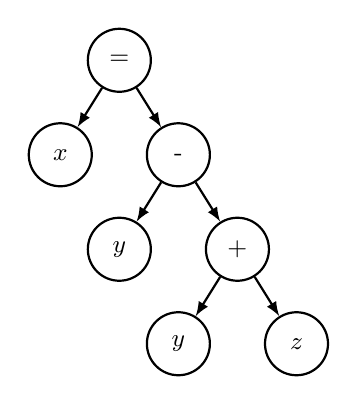
\begin{tikzpicture}[level distance=1.2cm, every node/.style={draw, circle, minimum size=0.8cm, font=\small}, thick,
          edge from parent/.style={draw, -latex},]
          \node {=}
            child { node {$x$} }
            child { node {-}
              child { node {$y$} }
              child { node {+}
                child { node {$y$} }
                child { node {$z$} }
              }
            };
        \end{tikzpicture}
    \end{center}

    \item 先写成三地址代码,如下所示:
    
    \begin{lstlisting}
        t1 = y + z
        t2 = y - t1
        x = t2
    \end{lstlisting}

    实现这个三地址代码的四元式序列如下表所示:
    \begin{center}
        \begin{tabular}{c|c|c|c|c|}
            \multicolumn{1}{c}{} & \multicolumn{1}{c}{$op$} & \multicolumn{1}{c}{$arg_1$} & \multicolumn{1}{c}{$arg_2$} & \multicolumn{1}{c}{$result$} \\
            \cline{2-5}
            0 & $+$ & y & z & t1 \\
            \cline{2-5}
            1 & $-$ & y & t1 & t2 \\
            \cline{2-5}
            2 & $=$ & t2 & & x \\
            \cline{2-5}
        \end{tabular}
    \end{center}

    \item 三元式序列如下所示:
    
    \begin{center}
        \begin{tabular}{c|c|c|c|}
            \multicolumn{1}{c}{} & \multicolumn{1}{c}{$op$} & \multicolumn{1}{c}{$arg_1$} & \multicolumn{1}{c}{$arg_2$} \\
            \cline{2-4}
            0 & $+$ & y & z \\
            \cline{2-4}
            1 & $-$ & y & (0) \\
            \cline{2-4}
            2 & $=$ & x & (1) \\
            \cline{2-4}
        \end{tabular}
    \end{center}

    \item 间接三元式序列如下所示:
    
    \begin{center}
        \begin{tabular}{c|c|}
            \multicolumn{2}{c}{$instruction$} \\
            \cline{2-2}
            35 & (0) \\
            \cline{2-2}
            36 & (1) \\
            \cline{2-2}
            37 & (2) \\
            \cline{2-2}
        \end{tabular}
    \end{center}
\end{enumerate}

\noindent
\tbf{8.3}

各个标识符的类型和相对地址如下表所示:

\begin{center}
    \begin{tabular}{|c|c|c|c|c|}
        \hline
        标识符 & 类型 & 大小 & 环境 & 相对地址 \\
        \hline
        x & float & 4 & 0 & 0 \\
        \hline
        p.x & float & 4 & 1 & 0 \\
        \hline
        p.y & float & 4 & 1 & 4 \\
        \hline
        p & record & 8 & 0 & 8 \\
        \hline
        q.m.tag & int & 4 & 2 & 0 \\
        \hline
        q.m.float & float & 4 & 2 & 4 \\
        \hline
        q.m & record & 8 & 1 & 0 \\
        \hline
        q.n.idx & int & 4 & 2 & 0 \\
        \hline
        q.n.y & float & 4 & 2 & 4 \\
        \hline
        q.n & record & 8 & 1 & 8 \\
        \hline
        q & record & 16 & 0 & 16 \\
        \hline
    \end{tabular}
\end{center}

\noindent
\tbf{8.4}

\begin{enumerate}[label=(\arabic*)]
    \item 该表达式的注释语法分析树如下所示:
    
    \begin{center}
    \scalebox{0.8}{
    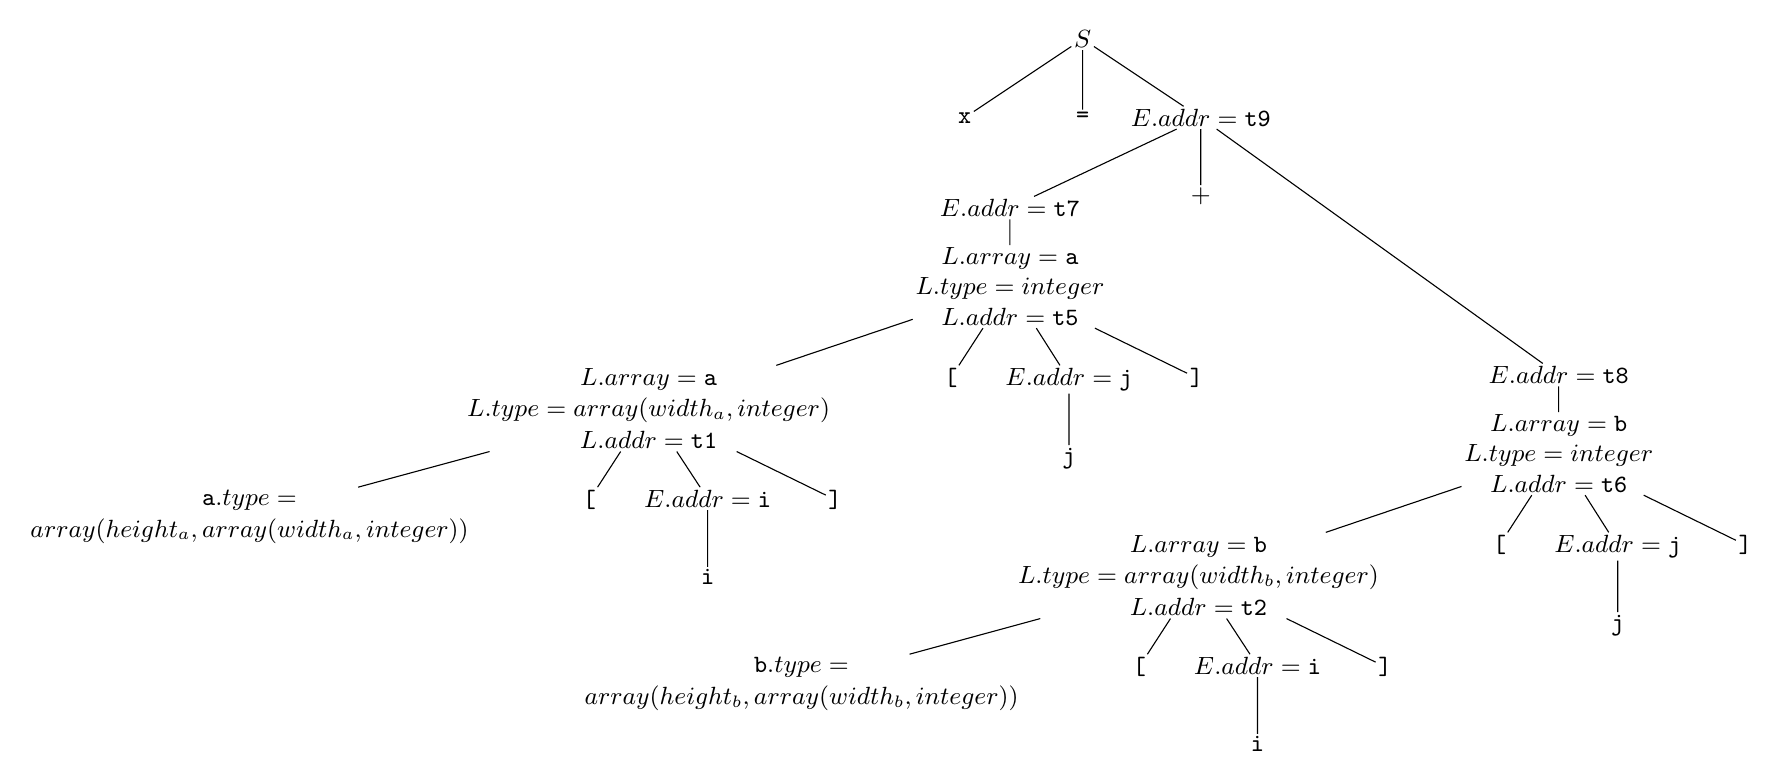
\begin{tikzpicture}[
        level distance=1cm,
        every node/.style={align=center, font=\small, inner sep=1pt, outer sep=0pt},
        grow=down
        ]
        \node {$S$}
            child {node {\texttt{x}}}
            child {node {\texttt{=}}}
            child {node {$E.addr = \texttt{t9}$}
                child {node[below left]{$E.addr = \texttt{t7}$}
                    child {node{\shortstack{$L.array = \texttt{a}$ \\
                                $L.type = integer$ \\
                                $L.addr = \texttt{t5}$}}
                        child {node[below left]{\shortstack{$L.array = \texttt{a}$ \\
                                    $L.type = array(width_a, integer)$ \\
                                    $L.addr = \texttt{t1}$}}
                            child {node[below left=]{\shortstack{$\texttt{a}.type =$ \\ $array(height_a, array(width_a, integer))$}}}
                            child {node[below]{\texttt{[}}}
                            child {node[below]{$E.addr = \texttt{i}$} 
                                child {node{\texttt{i}}}
                            }
                            child {node[below right]{\texttt{]}} }
                        }
                        child {node[below]{\texttt{[}}}
                        child {node[below]{$E.addr = \texttt{j}$} 
                            child {node{\texttt{j}}}
                        }
                        child {node[below right]{\texttt{]}} }
                    }
                }
                child { node{$+$} }
                child { node[below right=3cm]{$E.addr = \texttt{t8}$}
                    child {node{\shortstack{$L.array = \texttt{b}$ \\
                                $L.type = integer$ \\
                                $L.addr = \texttt{t6}$}}
                        child {node[below left, sibling distance=2.5cm]{\shortstack{$L.array = \texttt{b}$ \\
                                    $L.type = array(width_b, integer)$ \\
                                    $L.addr = \texttt{t2}$}}
                            child {node[below left=]{\shortstack{$\texttt{b}.type =$ \\ $array(height_b, array(width_b, integer))$}}}
                            child {node[below]{\texttt{[}}}
                            child {node[below]{$E.addr = \texttt{i}$} 
                                child {node{\texttt{i}}}
                            }
                            child {node[below right]{\texttt{]}} }
                        }
                        child {node[below]{\texttt{[}}}
                        child {node[below]{$E.addr = \texttt{j}$} 
                            child {node{\texttt{j}}}
                        }
                        child {node[below right]{\texttt{]}} }
                    }
                }
            };
    \end{tikzpicture}
    }
    \end{center}

    翻译成三地址代码如下所示:

    \begin{lstlisting}
    t1 = i * 4width_a
    t2 = i * 4width_b
    t3 = j * 4
    t4 = j * 4
    t5 = t1 + t3
    t6 = t2 + t4
    t7 = a[t5]
    t8 = b[t6]
    t9 = t7 + t8
    x = t9
    \end{lstlisting}

    \item 该表达式的注释语法分析树如下所示:
    
    \begin{center}
    \scalebox{0.8}{
    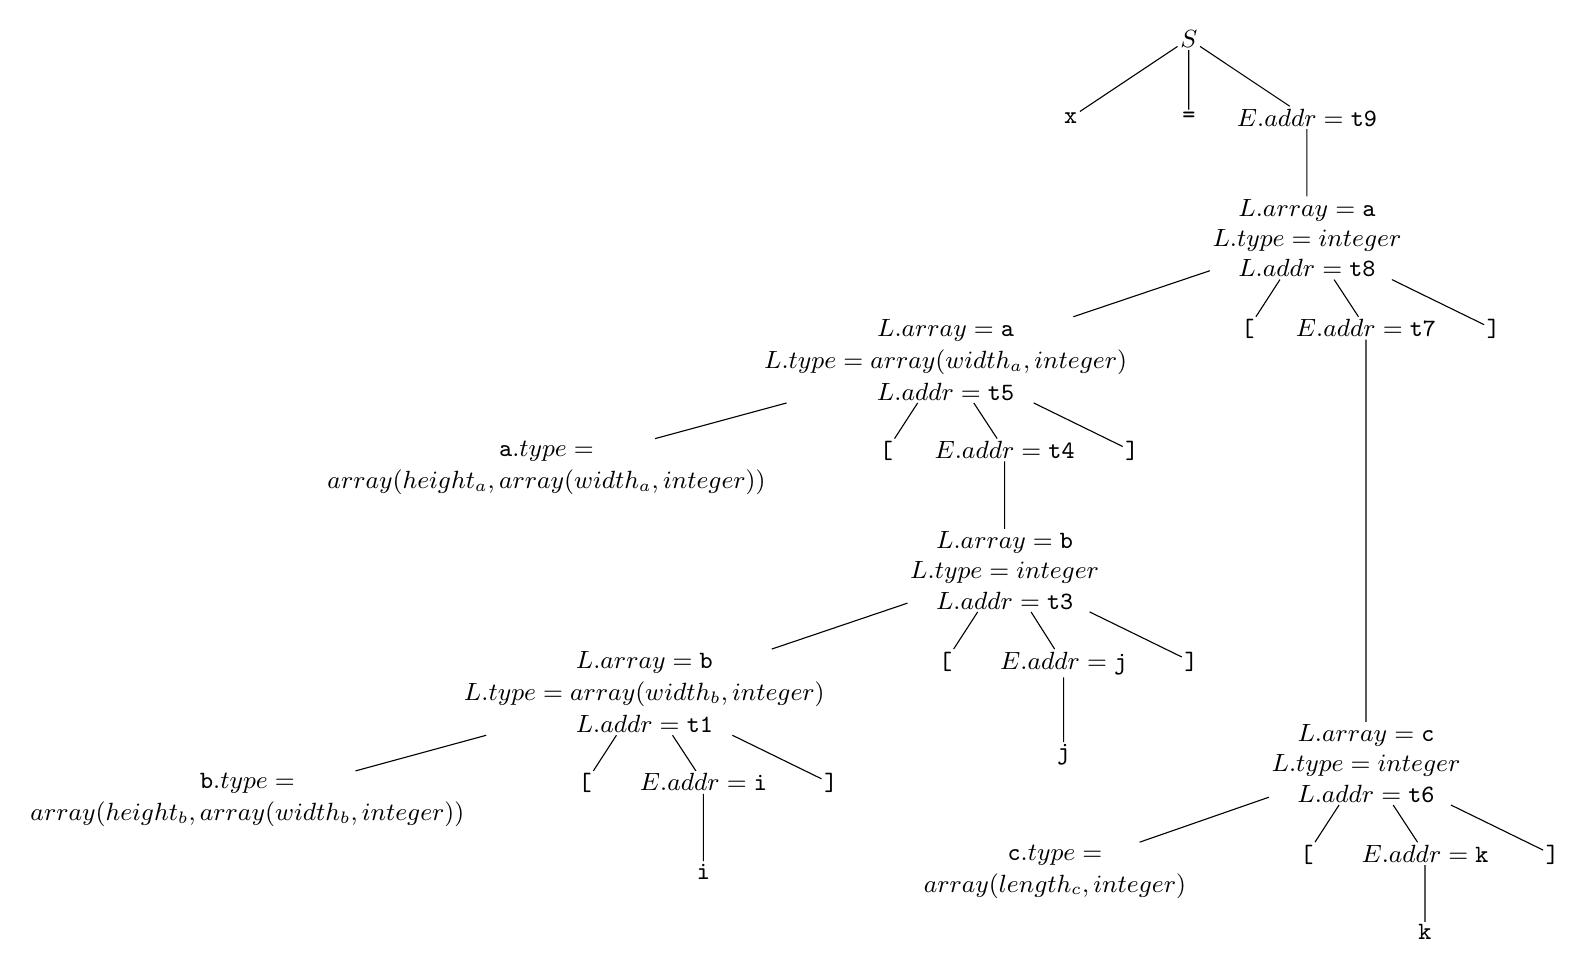
\begin{tikzpicture}[
        level distance=1cm,
        every node/.style={align=center, font=\small, inner sep=1pt, outer sep=0pt},
        grow=down
        ]
        \node {$S$}
            child {node {\texttt{x}}}
            child {node {\texttt{=}}}
            child {node {$E.addr = \texttt{t9}$}
                child {node[below]{\shortstack{$L.array = \texttt{a}$ \\ $L.type = integer$ \\ $L.addr = \texttt{t8}$}}
                    child {node[below left]{\shortstack{$L.array = \texttt{a}$ \\ $L.type = array(width_a, integer)$ \\ $L.addr = \texttt{t5}$}}
                        child {node[below left=]{\shortstack{$\texttt{a}.type =$ \\ $array(height_a, array(width_a, integer))$}}}
                        child {node[below]{\texttt{[}}}
                        child {node[below]{$E.addr = \texttt{t4}$} 
                            child[below=1cm]{node{\shortstack{$L.array = \texttt{b}$ \\
                                        $L.type = integer$ \\
                                        $L.addr = \texttt{t3}$}}
                                child {node[below left, sibling distance=2.5cm]{\shortstack{$L.array = \texttt{b}$ \\
                                            $L.type = array(width_b, integer)$ \\
                                            $L.addr = \texttt{t1}$}}
                                    child {node[below left=]{\shortstack{$\texttt{b}.type =$ \\ $array(height_b, array(width_b, integer))$}}}
                                    child {node[below]{\texttt{[}}}
                                    child {node[below]{$E.addr = \texttt{i}$} 
                                        child {node{\texttt{i}}}
                                    }
                                    child {node[below right]{\texttt{]}} }
                                }
                                child {node[below]{\texttt{[}}}
                                child {node[below]{$E.addr = \texttt{j}$} 
                                    child {node{\texttt{j}}}
                                }
                                child {node[below right]{\texttt{]}} }
                            }
                        }
                        child {node[below right]{\texttt{]}} }
                    }
                    child {node[below]{\texttt{[}}}
                    child {node[below]{$E.addr = \texttt{t7}$}
                        child {node[below=4cm]{\shortstack{$L.array = \texttt{c}$ \\ $L.type = integer$ \\ $L.addr = \texttt{t6}$}}
                            child {node[below left]{\shortstack{$\texttt{c}.type =$ \\ $array(length_c, integer)$}}}
                            child {node[below]{\texttt{[}}}
                            child {node[below]{$E.addr = \texttt{k}$} 
                                child {node{\texttt{k}}}
                            }
                            child {node[below right]{\texttt{]}} }
                        }
                    }
                    child {node[below right]{\texttt{]}}}
                }
            };
    \end{tikzpicture}
    }
\end{center}

翻译成三地址代码如下所示:

\begin{lstlisting}
t1 = i * 4width_b
t2 = j * 4
t3 = t1 + t2
t4 = b[t3]
t5 = t4 * 4width_a
t6 = k * 4
t7 = c[t6]
t8 = t5 + t7
t9 = a[t8]
x = t9
\end{lstlisting}
\end{enumerate}

\end{document}